\section{High-Level Usage}

HOOVER exposes a C/C++ API  to a SPMD programming model, inherited from the
OpenSHMEM programming model that it is built on top of. While most of the
application code does not need to be aware of the SPMD-ness of the underlying
runtime, application initialization is performed in parallel across all PEs in the
simulation. This choice was made deliberately so that large datasets could be
loaded across all PEs, rather than exposing sequential semantics by only
loading the dataset on a single PE and then broadcasting it.

The core data structure of HOOVER is a graph vertex. In HOOVER, a vertex can
have zero or more attributes attached to it, stored as a sparse
vector. During the execution of a HOOVER simulation, the user-level, application-specific
code is primarily responsible for reading and updating attributes
on local and remote vertices based on application-specific semantics.

Attributes in HOOVER are split into two categories: positional and logical.
Positional attributes on a vertex define its relationship and distance to other
vertices in the simulation. Positional attributes are used by HOOVER to
automatically update edges between vertices as they move ``closer'' or ``farther'' away.
For example, positional attributes might be the physical location of a
vertex in a 2D or 3D space, defining its location relative to other vertices.
Logical attributes are additional vertex attributes used by the
programmer for application-specific information, but which are not used by the
HOOVER runtime system.

At a high level, a HOOVER program starts with the user configuring a graph
problem by defining the initial state/attributes of all vertices in it. This
initial state is then passed into the HOOVER runtime along with several
application-specific callbacks. All future execution is then coordinated by the
HOOVER runtime, with application callbacks made when application-specific
behavior or updates are needed.

\begin{figure}
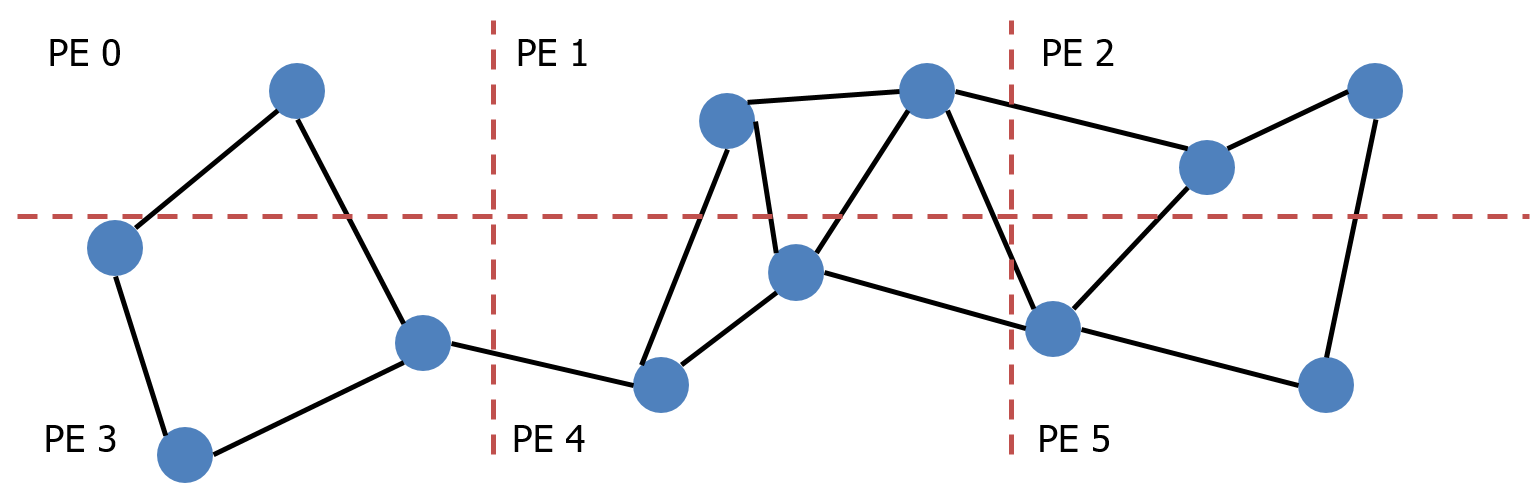
\includegraphics[width=\columnwidth]{pe_diag.png}
\caption{Illustration of a HOOVER graph distributed across PEs with cross-PE
    edges.}
\label{fig:pe_diag}
\end{figure}

\subsection{Target Application Pattern}

While HOOVER is a general dynamic graph processing, simulation, and analytics
framework it also offers specialized capabilities for a particular class of
dynamic graph problems. The classical HOOVER problem follows the following high
level execution flow:

\begin{enumerate}
    \item The application defines a large number of vertices partitioned across
        PEs, as well as callbacks to update their state (among other things).
    \item The HOOVER framework begins iterative modeling of vertex behavior
        through repeated callbacks to user-level functions, evolving vertex
        state over time. All PEs execute entirely de-coupled from each other.
        While each PE is asynchronously made aware of summaries of the state
        change in other PEs, no PE is ever blocked on or performing two-sided
        communication with any other PE.
    \item After some time, two or more PEs discover they are related. This
        ``relationship'' is entirely user-directed and in the control of user
        callbacks. After this connectivity is discovered, those PEs will enter
        lockstep execution with each other and share data on each timestep.
        Multiple clusters of coupled PEs may evolve over time, with separate
        groups of PEs becoming interconnected or all PEs evolving into a single,
        massive cluster depending on the application.
    \item Eventually, application termination is either signalled by a PE or
        controlled by all PEs reaching a maximum number of timesteps.
\end{enumerate}

At this point, an illustrative example might be useful: malware spread over
Bluetooth. Malware propagation modeling can be expressed as a graph problem,
where vertices in the graph represent Bluetooth devices and edges represent direct
connectivity between two devices. Executing malware propagation on the
HOOVER framework might look something like:

\begin{enumerate}
    \item The application developer would define the actors in the simulation as
        vertices passed down to the HOOVER framework. Each actor would represent
        a device, and may include attributes such as the range of its Bluetooth
        hardware, the model its Bluetooth hardware, the speed at which it can
        move, or its initial infected/uninfected status.
    \item HOOVER would then begin execution, updating device infection status,
        position, and connectivity with other devices based on user callbacks and
        other information passed in by the application developer. As iterations
        progress, more and more devices might become infected from a small
        initial seed of infected devices.
    \item Eventually, two or more PEs may become coupled at the application
        developer's direction. For example, the developer might instruct two PEs
        to become coupled if a device resident on one PE infects a device resident
        on another. By entering coupled, lockstep execution those two PEs can
        now compute several joint metrics about the infection cluster they
        collectively store, such as number of infected devices or rate of
        infection progression. Note that even when PEs create a tightly coupled
        cluster, they still interact as usual with any other PEs in the
        simulation which they are not coupled with.
\end{enumerate}
